\chapter{Robust handling of enduring contacts}
\label{ch:RobustHandlingofSlidingContacts}
This chapter outlines the artifacts we observed emerging from the CPF algorithm \cite{TANG2012} and our approaches to treat them. We will first give a brief overview on the artifacts and then describe them in detail. Subsequently, we will describe our approaches to handle the artifacts.

\section{CPF Artifacts}
\label{sec::CPFArtifacts}
The CPF collision handling as described by Tang et al. \cite{TANG2012} shows artifacts, in particular for enduring contacts. Enduring contacts are contacts, which are not resolved in the time step they occur. We observed three major artifacts, separated features still assumed colliding, additional artificial collisions through discretization and inconsistent feature pair mapping. The artifacts emerge if collisions from previous time steps are not completely resolved and additionally a colliding features performs a motion tangential to the surface it is intersecting. In particular, such a behavior can be observed for sliding and deep collisions.

\subsection{Separated Features Still Assumed Colliding}
\label{ss:ResolvedCollisionsRemain}

\begin{figure}[h!] 
  \centering
     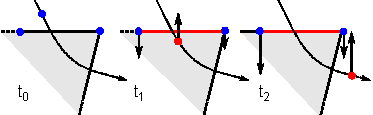
\includegraphics[width=0.75\textwidth]{pics/pdf/slidingVertexArtifactUnresolvedCollision.pdf}
  \caption[2D-Illustration of a VF collision, which is considered colliding after it is already resolved]{2D-Illustration of a VF collision, which is considered colliding after it is already resolved. Dots indicate the vertices, the red ones are colliding. The straight lines indicate the the surface triangles, the red ones are colliding. The black arrows indicating the applied impulses.  $t_0$ no collision; $t_1$ the single vertex is colliding with the red triangle; $t_2$ the single vertex is still colliding with the red triangle, although it left the body through the black face.}
  \label{fig:slidingVertexArtifactUnresolvedCollision}
\end{figure}

A feature pair is considered colliding as long as the penetration depth is strictly negative \cite{TANG2012}.
This can lead to feature pairs, which are considered colliding even 
if the bodies are already separated.
The collision resolution is missed if a feature is colliding with another feature and leaves the body by passing through a third feature, without reducing the original penetration depth to zero. A good example for such a scenario is shown in figure \ref{fig:slidingVertexArtifactUnresolvedCollision}. A vertex enters a cube through the top face and leaves the cube through a side face, however the separated features are still assumed to be colliding.

For EE collisions a similar behavior can be observed. For EE collisions it is additionally possible that an edge leaves the body without colliding with another edge.



\subsection{Additional Artificial Collisions Through Discretization}
\label{ss:DiscretizationCollisonForces}

Consider a cube colliding with an analytical static plane. Correctly there are only impulses applied to the object in the direction normal to the plane and the cube's tangential velocity does not change.
If we swap the analytical plane for a discretized triangle surface mesh, again we would expect that only impulses are applied which show in the direction normal to the plane. 
However, collisions arise with normals showing in a direction tangential to the plane. They stop the tangential movement directly and and hook the body in the surface, as shown in figure \ref{fig:slidingVertexArtifactDiscretizationForces}. These collisions arise between the edges and vertices of the plane with the edges and faces of the cube. However, the edges and vertices of the plane are only a product of the discretization and should not induce tangential forces.

The artifact can be described more generic as follows. When two bodies collide with non-zero tangential velocity or with deep intersections, collisions arise with contact normals showing in a direction tangential to the surfaces. This makes the objects collide sidewards, stops the tangential movement and hooks the objects between surface elements.

In our simulations the consequences of this artifact were severe to such an extent that a simulation of collisions with even only small tangential movement was not possible.
\begin{figure}[h] 
  \centering
     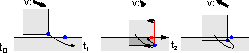
\includegraphics[width=0.95\textwidth]{pics/pdf/slidingVertexArtifactDiscretizationForces.pdf}
  \caption[2D-Illustration of a hooked VF collision with tangential forces induced by the CPF algorithm.]{2D-Illustration of a hooked VF collision with tangential forces induced by the CPF algorithm. For the sake of clarity, only the artifact collision is highlighted.  $t_0$ no collision; $t_1$ the red face collides with the surface vertex of the lower body resulting in forces almost tangential to the surface of the lower body and reverting the tangential movement; $t_2$ the artifact collision is resolved, however the colliding object completely reverted its velocity, similar to a collision with a artificial wall.}
  \label{fig:slidingVertexArtifactDiscretizationForces}
  

\end{figure}


\subsection{Inconsistent Feature Pair Mapping}
\label{ss:ImplausibleFeaturePairs}
When two features collide, the feature pair and the barycentric weights are stored for further collision treatment and used until the collision is resolved \cite{TANG2012}.

 For the VF case, this can lead to implausible feature pairs when a vertex moves tangential to the surface of the body it is intersecting.
The implausible feature pairs arise if the vertex continues its tangential movement and moves below a neighboring triangle, as shown in Fig \ref{fig:slidingVertexArtifactImplausibleForces}. As a result there are large distances between the vertex and the colliding triangle, which results in impulses at distant vertex positions. This leads to implausible behavior as an object is deformed at positions distant from the collision.

\begin{figure}[h!] 
  \centering
     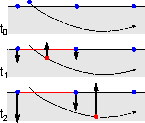
\includegraphics[width=0.4\textwidth]{pics/pdf/slidingVertexArtifactImplausibleForces.pdf}
  \caption[2D-Illustration of a VF collision causing impulses at implausible positions.]{2D-Illustration of a VF collision causing impulses at implausible positions.
  At time $t_0$ there is no collision. At time $t_1$ the single vertex is colliding with the red triangle. At time $t_2$ the single vertex is still colliding with the red triangle, although the vertex shifted under the triangle right to the red one.}
  \label{fig:slidingVertexArtifactImplausibleForces}
\end{figure}

In the case of EE collisions, a similar behavior can be observed. When an edge moves tangential to the surface of the body it is intersecting and the edge slides below another edge, impulses are applied at distant positions. 

Furthermore, the implausible feature pairs can lead to wrong resolutions of collisions, as shown in figure \ref{fig:slidingVertexSmallRotation}. With a large distance between the two colliding features, only a minor rotation of the colliding face or an colliding edge is necessary to reduce the penetration depth to zero. Thereby the resolution condition (given in section \ref{sec:CCDandPenetrationDepth}) is fulfilled, whereas the feature might still be intersecting the body.
\begin{figure}[h] 
  \centering
     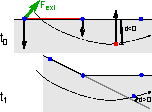
\includegraphics[width=0.4\textwidth]{pics/pdf/slidingVertexSmallRotation.pdf}
  \caption[2D-Illustration of an incorrect VF collision resolution artifact]{2D-Illustration of an incorrect VF collision resolution artifact. At time $t_0$ the single vertex is colliding with the red triangle and a external force is applied to the red triangle. At time $t_1$ the red triangle rotated, the distance of the vertex to the triangle plane is now positive and thereby the collision resolution condition is incorrectly satisfied.}
  \label{fig:slidingVertexSmallRotation}
\end{figure}
This unwanted resolution appears for example when a rigid cube is dropped on a deformable bar and afterwards the rigid cubes slides on the bar. Due to impact of the rigid body, the surface of the deformable body oscillates and the surface triangles perform small rotations. These rotations are sufficient to fulfill the resolution condition. Thereby the collision is "resolved", whereas the vertex should still be colliding since it is intersecting the body.


\section{CPF Extensions}
\label{sec::CPFExtensions}
To maintain plausible feature pairs and correct resolution impulses, extensions of the original CPF algorithm are necessary.
In total we introduce three additional steps solving and reducing the issues described in the previous section. % as described in detail in the following. %:
%To solve the resolved collisions remaining we introduce an advanced resolution condition.
%To handle the implausible feature pairs we introduce a redefinition algorithm.
%To prevent the discretization collision forces, we categorize the contacts in regular, sliding or hooked and treat the collisions accordingly.


\subsection{Advanced Resolution Condition}
\label{ss:AdvResCond}
To accomplish a correct resolution detection and to avoid the separated features still assumed colliding, we extend the resolution condition by additionally taking collisions of the features' vertices into account.

For the VF case, we consider a collision resolved, if either the penetration depth is positive or the colliding vertex collides with another face of the intersecting body. This condition is sufficient, since no collision is missed due to the CCD. Therefore, when the collision resolves the vertex passes the surface of the body it is intersecting and thereby a triangle vertex contact is detected. 

For the EE case we consider a collision resolved, if either the penetration depth is positive or when both vertices of an edge are resolved and the edge is not intersecting a face of the previously intersected body.
This condition is sufficient, since when the edge is colliding, but none of the edge's vertices is colliding, the edge pierces the surface and thereby the edge intersects a triangle. Otherwise, the edge is not colliding.

\subsection{Contact Categorization}
\label{ss::ContactCategorization}
As described in section \ref{ss:DiscretizationCollisonForces}, some collisions generate artifact forces when the tangential velocity is non-zero. To avoid the artifact forces we need to distinguish these collisions from the regular collisions. Therefore, we introduce conditions in order to categorize the collisions either as "regular", which can be handled with the regular algorithm or as "hooked", which generate artifact forces and require special handling. The categorization is limited to non-deep contacts, though we will discuss possibilities to extend the categorization to deep collisions at the end of the section.

A \textbf{regular} collision is considered as the common case, with the two bodies being pushed away from each other. This applies for collisions with the surface normals of the colliding features showing in opposite directions and the resolution impulses showing inside the according bodies. Regular collisions are handled with the original algorithm.

A \textbf{hooked} collision appears for sliding contacts or deep intersections. The surface normals are closer to an orthogonal state than to an opposing state. This results in impulses tangential to a surface. These collisions are implausible since the tangential motion should not change without friction. The body hooks in the surface, as it can be seen in figure \ref{fig:slidingVertexArtifactDiscretizationForces}.
Therefore, we redefine the feature pairs of hooked collisions in order to reduce the tangential impulses and to gain regular collisions.

In the following we will discuss the formulation with an emphasis on the VF case. Afterwards, we will give the definition for the EE case, which is analogous.

The previous description yields the basic formulation of the condition for a hooked collision:  A collision is hooked, if the proportion of the contact normal  $\mathbf{n_{c}}$ in a direction tangential to the surface of a feature is larger than the proportion in the direction normal to the surface. Otherwise, the collision is regular. The contact normal is equal to the direction of the applied collision impulse. To express the surface direction of a vertex, we apply the averaged vertex normal $\mathbf{n_{v}}$ as the average of the adjacent face normals and handle it as a surface normal. The condition for a hooked collision can now be expressed with the dot product as
\begin{equation}
-\mathbf{n_{v} \cdot n_{c}}<\cos(45^\circ)=\frac{\sqrt 2}{2},
\end{equation}
with a negative sign before the dot product since the two normals are opposing.
This relation is illustrated in the classification circle, see figure
\ref{fig::classification}. It is not necessary to additionally check the triangle normal against the contact normal since the contact normal is equal to the triangle normal. Thereby, they are per definition always showing in the same direction.
\begin{figure}[tbp] 
  \centering
     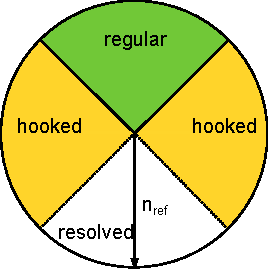
\includegraphics[width=0.4\textwidth]{pics/pdf/classification.pdf}
  \caption[2D-Illustration of the classification circle.]{The classification circle is an illustration of the condition for a hooked collision. Depending on the surface normal $n_v$, as shown as example by the grey arrow, and the fixed contact normal $\mathbf n_c$it is possible to determine whether a collision is hooked or regular.}
  \label{fig::classification}
\end{figure}
\begin{figure}[tbp] 
  \centering
     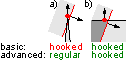
\includegraphics[width=0.55\textwidth]{pics/pdf/anglesOfAttack.pdf}
  \caption[Comparison of the contact categorization with normals and normal spans.]{Comparison of collisions of vertices in acute-angled and an obtuse-angled corners. The subfigures a) and b) have the same relation between the contact normals and the averaged vertex normal. Therefore, the basic formulation yields that both collisions are hooked. However, for a) the contact normal is almost parallel to the two face normals, therefore we would expect an regular collision.}
  \label{fig::anglesOfAttack}
\end{figure}

The basic formulation is insufficient for vertices in acute-angled corners, as shown in the following.
Vertices in acute-angled corners of a tetrahedron can collide in a larger area of contact angles than vertices in obtuse-angled corners, as shown in figure \ref{fig::anglesOfAttack}.  The figure compares collisions of vertices in acute-angled and an obtuse-angled corners. The subfigures a) and b) have the same relation between the contact normals and the averaged vertex normal. Therefore, the basic formulation yields that both collisions are hooked. However, for subfigure a) the contact normal is almost parallel to the two face normals, therefore we would expect a regular collision. Furthermore, the angle between the averaged vertex normal the normal of the adjacent faces is large, it is close to $90^\circ$. Thereby, the averaged vertex normal does not provide a sufficient expression of the surface normal for acute-angled corners.


Therefore, we need to introduce a construct taking the angles between adjacent face normals into account.
 Accordingly, we introduce a cone alike span $\mathbf{N}$ (see figure \ref{fig::vertexNormalSpan}) spanned by the surface normals of the directly adjacent faces of the vertex or edge. It will be called "normal span" in the following. 
\begin{figure}[h] 
  \centering
     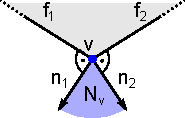
\includegraphics[width=0.4\textwidth]{pics/pdf/vertexNormalSpan.pdf}
  \caption[2D-Illustration of the vertex normal span $\mathbf{N_v}$ of the vertex v.]{2D-Illustration of the vertex normal span $\mathbf{N_v}$ of the vertex v. The normals of the faces $\mathbf{f_1}$ and $\mathbf{f_2}$ are indicated $\mathbf{n_1}$ and $\mathbf{n_2}$. The vertex normal span is indicated in light blue.}
  \label{fig::vertexNormalSpan}
\end{figure}
The normal span is large for acute-angled corners and small for obtuse-angled corners. Thereby, the normal span reflects the collision behavior for vertices in such corners and a proper contact categorization is possible (see figure 
\ref{fig::vertexNormalSpanComp}). The illustration compares the collision category evaluation for the collisions with averaged normals and normal spans. It emphasizes that with normal spans an accurate collision categorization can be provided, regardless of the angle in the vertex corner.
\begin{figure}[h] 
  \centering
     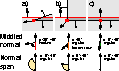
\includegraphics[width=0.65\textwidth]{pics/pdf/stupidNormals2.pdf}
  \caption[Comparison of the contact categorization with normals and normal spans for VF collisions with the vertex in an acute-angled, right-angled and obtuse-angled corner.]{Comparison of the contact categorization with normals and normal spans for VF collisions with the vertex in an acute-angled, right-angled and obtuse-angled corner. a) shows a acute-angled corner of a tetrahedron colliding with a flat surface. The normal span indicates correctly a regular collisions, in contrast to the normals indicating a hooked collision.  b) shows a  right-angled corner of a cube colliding with a flat surface. The normal span indicates correctly a regular collisions, for the normals it is exactly the border between hooked and valid.  c) shows a vertex of a flat surface colliding with a flat surface. Both, the normal span and the normals indicate the collision correctly as regular.}
  \label{fig::vertexNormalSpanComp}
\end{figure}

To implement the normal span in the simulation, we need to discretized it.
Therefore, we approximate the normal span by the set of triangle normals adjacent to the vertex or edge.
For edges only the two directly adjacent faces are considered. For the approximation of larger normal cones we additionally add the averaged vertex normal to the set.


For the contact categorization the normal cone is an often used element.
To avoid a large computation overhead due to searching of neighboring elements in order to compute their normal, it is necessary to apply a data structure providing fast neighborhood information. 
We use a data structure by Serna et al. \cite{SERNA2009B} providing the necessary fast neighborhood information.


The previously introduced category definitions are implemented as follows. 
A VF collision is hooked, if the proportion of the contact normal showing in the direction tangential to the vertex surface is larger than proportion showing in the normal direction, expressed similar to the basic formulation as
\begin{equation}
\min(\mathbf{\{n_{Vi} \cdot n_{cv}\}})>-\frac{\sqrt 2}{2} \; | \; \mathbf{n_{Vi}} \in \mathbf{N_{v}},
\end{equation} with the normal span of the vertex $\mathbf{N_{v}}$ and the contact normal $\mathbf{n_{cv}}$. This formulation is similar to measuring the minimum angle between the normal span and the negative contact normal. If this angle is larger than $45^\circ$ the impulse proportion tangential to the face is larger than normal proportion and the collision is hooked.
Otherwise the collision is regular.


A EE collision is hooked,  if the proportion of the contact normal showing in the direction tangential to the surface is larger than proportion showing in the normal direction for both edges, expressed similar to the basic formulation as
\begin{equation}
\min(\mathbf{\{{n}_{Eai}\cdot{n}_{ce}\}})>-\frac{\sqrt 2}{2} \; \land  \; \max(\mathbf{\{{n}_{Ebi}\cdot{n}_{ce}\}})<\frac{\sqrt 2}{2} \; | \;, \mathbf{n_{Eai}} \in \mathbf{N_{Ea}},\; \mathbf{n_{Ebi}} \in \mathbf{N_{Eb}}
\end{equation} with the normal spans $\mathbf{N}_{Ea}$ and $\mathbf{N}_{Eb}$ of the edges and the contact normal $\mathbf{n_{ce}}$.

If the collision is not hooked, it is regular.

The handling of regular collisions is straightforward. Regular collisions are handled with the CPF algorithm without modification. The handling on hooked contacts is based on the algorithm for the redefinition of feature pairs in the next section \ref{ss::redef}. Therefore, the handling of hooked contacts is described in section \ref{ss::sliding}.

In the beginning of this section we have stated that the categorization is only applicable for non-deep collisions. Now we will investigate the problem arising from deep collisions and how it could be solved.

This collision definition is limited to non-deep intersections, since we can not differentiate between a hooked contact and a deep intersection with only the local collision data, see figure \ref{fig::limitCategory}. On the left side the local collision arrangement is shown and on the right side three possible global arrangements for the  local collision arrangement are shown. With only the local collision data it is not possible to differentiate between the three cases.
\begin{figure}[h] 
  \centering
     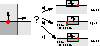
\includegraphics[width=0.75\textwidth]{pics/pdf/limitCategory.pdf}
  \caption[Illustration of limitation to of the algorithm to non-deep contacts.]{Illustration of limitation to of the categorization algorithm to non-deep contacts, since otherwise the collision arrangement is ambiguous, as shown by the possible arrangements a)-c).}
  \label{fig::limitCategory}
\end{figure}
 However, it is necessary to differentiate between the three cases in order to yield a distinct categorization since arrangements a) and c) are hooked collisions whereas b) is a regular collisions.
 As an interim solution we restricted the algorithm to non-deep collisions, thereby only arrangement a) is possible and the local arrangement is unambiguous. Furthermore, non-deep collisions are sufficient in many cases, since deep collisions often provide a visually unsatisfying result. 
  
 Nevertheless, the capability to handle deep contacts is desirable in order to simulate high-resolution meshes and to increase the overall robustness of the algorithm. To handle deep contacts additional information about the collision arrangement is required. This additional information could be provided by a global intersection analysis, similar to Baraff et al. \cite{BARAFF2003}, thereby it would be possible to differentiate between the sliding and the regular collisions for deep collisions. Alternatively, checking the neighbors of the new colliding vertex for collisions and taking their contact normals as a reference, would provide the necessary information and would provide less computational overhead.
 

\subsection{Redefinition of Feature Pairs}
\label{ss::redef}
%valid hier und valid by categories sollte unterscheidbar sein
To ensure plausible feature pairs and to avoid an inconsistent feature pair mapping, we trace the collisions and check each simulation step for possibly necessary redefinitions. A redefinition is possibly necessary if the first feature of the feature pair projected onto the second feature does not provide a geometrical overlap.
A redefinition is only "possibly" necessary since for concave surfaces it is possible that the projections of a feature do not overlap with any other feature. Imagine the 2D case of a vertex in the center of a five-pointed star, none of the sides overlaps with the projection of the vertex on the lines defined by the sides.

For VF collisions the assumption holds that as long as a vertex intersects a body, it is colliding with exact one face of the intersecting body. The redefinition for the VF case can be subdivided into two steps. The first step is to check if a redefinition is possibly necessary. If a redefinition is possibly necessary, we apply a second step and search for the correct face corresponding to the colliding vertex. 
An example of a VF redefinition is presented in figure \ref{fig::slidingVertexArtifactImplausibleForcesRedef} and in figure \ref{fig::svf_redef}.

In contrast to the VF case, no similar assumption holds for the EE case. An edge intersecting with another body can be colliding with one edge, with multiple edges or even with no edge.
Hence, there is no coherence between the elimination and new definition of a feature pair.
Therefore, the elimination and new definition are treated separately.
We check for eliminations at the end of each simulation step. For the new EE definitions we leverage that the new EE definitions go along with VF redefinitions.
Thus, we check for new EE definitions whenever we redefine a VF collision.

\begin{figure}[h] 
  \centering
     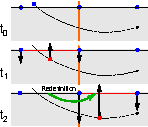
\includegraphics[width=0.40\textwidth]{pics/pdf/slidingVertexArtifactImplausibleForcesRedef.pdf}
  \caption[2D-Illustration of a barycentric redefinition.   Dots indicate the vertices, the red ones are colliding.]{2D-Illustration of a barycentric redefinition.   $t_0$ no collision, $t_1$ the single vertex is colliding with the left triangle, indicated red, $t_2$ the single vertex is now still colliding with the right triangle. The colliding face was redefined as indicated by the green arrow. The redefinition border is indicated with the orange-dotted line.}
  \label{fig::slidingVertexArtifactImplausibleForcesRedef}
\end{figure}


\begin{figure}[h!] 
\begin{minipage}[b]{0.5 \linewidth}
		\centering
		\subfigure[before the redefinition]{
			       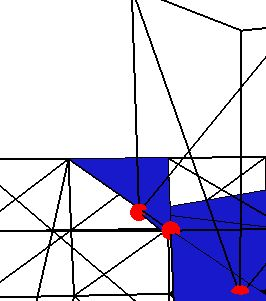
\includegraphics[width=0.4\linewidth]{pics/png/svf_redef_1.jpg} }
	\end{minipage}
	\begin{minipage}[b]{0.5 \linewidth}
		\centering
		\subfigure[after the redefinition]{
			       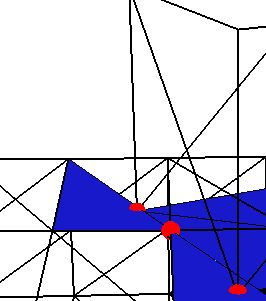
\includegraphics[width=0.4\linewidth]{pics/png/svf_redef_2.jpg} }
	\end{minipage}

  \caption[Example of a barycentric redefinition in a simulation.]{Example of a barycentric redefinition in a simulation. Subfigure a) shows the situation before the redefinition. Subfigure b) shows the same situation one time step later. The left vertex shifted under the next face, the collision is redefined and thereby updated to the next face .}
  \label{fig::svf_redef}
\end{figure}

\paragraph{Vertex Face Case}
For the VF case, we project the colliding vertex $V$ onto the plane of the colliding face $F$ and compute the barycentric coordinates $\omega_{fa}$, $\omega_{fb}$ and $\omega_{fc}$, see algorithm \ref{alg::VertexFaceFeaturePairRedefinition}.
The projected vertex is within the triangle if all barycentric weights are positive. Such collision pairs are considered valid and no redefinition is necessary.
Otherwise, it is possibly necessary to redefine the pair and we assume that the vertex went on to a face adjacent to the initial face.
With the direction information of the previously computed barycentric coordinates, we only need to check the faces adjacent to the vertices with positive weights.
Therefore, we project the vertex $V$ on the faces adjacent to vertices with positive weights.
 
Again, we check if the projected vertices are inside the new triangles by computing the barycentric weights.
All faces $F_i$ having only positive barycentric weights are candidates for the redefinition. In order the gain a regular collision, we apply the classification (see section \ref{ss::ContactCategorization}) and keep only the regular collisions as candidates. For the remaining candidates, we compute the penetration depths and choose the candidate with the smallest penetration depth. If no candidate was found, we do not redefine the collision.
 
To handle concave faces, we need to extend the algorithm.
For concave meshes it is possible that there is no face giving positive barycentric weights in the direct neighborhood. So we need to modify the barycentric weight condition. We define the barycentric tolerance $\varepsilon_v$ as
\begin{equation}
\varepsilon_v= \max\{
\begin{cases}
-\omega_i & \text{if } \omega_i<0 \\
\omega_i-1 &  \text{if } \omega_i>1\\
0&  \text{else}
\end{cases} \; | \; \omega_i \in \{\omega_a,\omega_b,\omega_c\}\}
\end{equation}
with the initial barycentric weights $\omega_{fa}$, $\omega_{fb}$ and $\omega_{fc}$.  $\varepsilon_v$ expresses the maximum discrepancy of the barycentric weights to the valid interval $[0,1]$.

In the algorithm we modify the condition for redefinition candidates. We now do not only add all vertices having all their barycentric coordinates in the interval $[0,1]$, but also the vertices in the interval $[-\varepsilon_v,1+\varepsilon_v]$.




\begin{algorithm}                    % enter the algorithm environment
\caption{Vertex Face Feature Pair Redefinition for convex meshes}          % give the algorithm a caption
\label{alg::VertexFaceFeaturePairRedefinition}                           % and a label for \ref{} commands later in the document
\begin{algorithmic}[1]                    % enter the algorithmic environment
    \STATE Input: Vertex V, Face F, List Collisions, List ResolvedCollisions,  $\omega_{FA}$, $\omega_{FB}$, $\omega_{FC}$, $n_F$
    \STATE Result:  List Collisions, List ResolvedCollisions
    	\STATE List RedefinitionCandidates
        \IF{$\omega_{FA}>0$}
           	\STATE RedefinitionCandidates.add(neighbouringFaces($V_A$))
        \ENDIF
        \IF{$\omega_{FB}>0$}
          	\STATE RedefinitionCandidates.add(neighbouringFaces($V_B$))    
        \ENDIF
        \IF{$\omega_{FC}>0$}
	        \STATE RedefinitionCandidates.add(neighbouringFaces($V_C$)) 
       	\ENDIF
       	\STATE currentBestDepth $=-\infty$ 
       	\STATE Collision currentCollision
       	\FORALL{Face $F_i$ in RedefinitionCandidates}
       	 	\STATE $\omega_{IA}$, $\omega_{IB}$, $\omega_{IC}$ $ \Leftarrow$ computedProjectedBarycentrics(V,$F_i$)       	  	
	        \IF{$\omega_{IA}>0 \land \omega_{IB}>0 \land \omega_{IC}>0$}
	        \IF{regular==collisontype(Collision(V,$F_i$))}
     	       	\STATE $n_i =$faceNormal($F_i$) 
     	    	\STATE $d_i$ =penetrationdepth(V,$F_i)$
	        	\IF{$d_i>$currentBestDepth $\land$ $d_i<0$)}
					\STATE currentBestDepth$=d_i$
					\STATE currentCollision$=$Collision(V,$F_i$)				
							  		\ENDIF 			
							  				  		\ENDIF 
	     	\ENDIF
        \ENDFOR
     	\IF{currentBestDepth$>-\infty$}
	     	\STATE Collisions.add(currentCollision)
	     	\STATE ResolvedCollisions.add(Collision(V,F))
     	\ENDIF
\end{algorithmic}
\end{algorithm}


\paragraph{Edge Edge Case} For the EE case, in each simulation step before we compute the collision impulses, we check whether the collision needs to be dismissed. Therefore, we project the edge $E_B$ on the plane defined by the Edge $E_A$ with the contact normal as plane and projection normal. We compute the barycentric coordinates $\omega_{A0}$, $\omega_{A1}$, $\omega_{B0}$ and $\omega_{B1}$  of the point of intersection between the projected $E_A$ with $E_B$.
If the edges overlap, all barycentric coordinates are positive and the collision will be handled.
To avoid the missing of EE collisions, we apply a relaxed condition; if the barycentric weights are in the interval $[-\varepsilon_E,1+\varepsilon_E]$ with $\varepsilon_E=0.3$ the collision is kept, but not handled. For the case that not even the relaxed condition is fulfilled, the collision is dismissed.

Due to the circumstance that there is not always a coherence between the dismissing of an EE collision and the appearance of a new EE collision, checking the dismissed edges' neighbors is not sufficient for an accurate EE redefinition.
In consideration of the circumstance that EE redefinitions go along with VF redefinitions we couple the EE redefinitions to the VF redefinitions instead of EE dismissals.

We consider a VF redefinition of a vertex $V_S$ which is redefined from the face $F_{old}$ with the face normal $n_{ref}$ to the adjacent face $F_{new}$. All neighboring edges of $V_S$ are saved in a candidate list $L_A$. All edges adjacent to at least one of the mutual vertices of  $F_{old}$ and $F_{new}$ are saved in a second candidate list $L_B$. 

%Both lists are filtered to ensure plausible feature pairs.
%For $L_A$ we only allow edges with a surface normal span showing in the opposite direction of $n_{ref}$ and the edge vector orthogonal to $n_{ref}$. For $L_B$ the filter is similar, except that surface normal span has to show in the same direction as $n_{ref}$.
 
We test all possible EE feature pairs for new collisions, by testing each edge in $L_A$  against each edge in $L_B$. If a feature pair is according to section \ref{ss::ContactCategorization} regular and the projected barycentric coordinates are in the relaxed interval $[-\varepsilon_E,1+\varepsilon_E]$ we keep the feature pair as a collision.


\subsection{Redefinition of Hooked Contacts}
\label{ss::sliding}

We consider hooked collisions as aberrant and correct these collisions.
A nearby attempt would be to directly modify the direction of the collision impulse.
However, the direction is defined by the contact normal, which is an essential element of the CPF algorithm. Therefore, we redefine the hooked collision pairs in order to reduce the tangential impulses and to gain regular collision pairs, as shown in figure \ref{fig::slidingVertexArtifactDiscretizationForcesRedef}.
For the EE case these redefinitions are already covered by the collision redefinition in section \ref{ss::redef}. 
For the VF case we handle the hooked contacts with a redefinition of the feature pair similar to the implausible feature pairs case, see section \ref{ss::redef}.
In contrast to the implausible feature pairs case, the barycentric weights for the initial face generally are positive.
This allows us to use algorithm \ref{alg::VertexFaceFeaturePairRedefinition} with only a small change in the first step. We now search in all triangles adjacent to the triangle vertices and not only the triangles adjacent to vertices with positive weights. This change is necessary since we do not have a direction information, as in the case of barycentric redefinition provided by violation of [0,1] interval by the barycentric weights. 

\begin{figure}[h] 
  \centering
     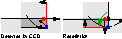
\includegraphics[width=0.70\textwidth]{pics/pdf/slidingVertexArtifactDiscretizationForcesRedef.pdf}
  \caption[2D-Illustration of the redefinition for a hooked collision.]{2D-Illustration of the redefinition for a hooked collision. The redefinition is marked with a green arrow. Before the redefinition, the red face collides with the surface vertex of the lower body resulting in forces almost tangential to the surface of the lower body and reverting the tangential movement. After the redefinition, the vertex collides with the redefined bottom sided face, resulting in forces in the normal direction of the lower surface and the tangential movement is preserved.}
  \label{fig::slidingVertexArtifactDiscretizationForcesRedef}
\end{figure}

In sum, the redefinition algorithm for a hooked collision can be reduced to four (simplified) steps (see figure \ref{fig::slidingVertexArtifactDiscretizationForcesRedefAlgo}). In the first step, the triangles adjacent to the colliding triangle are saved as candidates. In the second step, the colliding vertex is projected onto the planes defined by the candidate triangles and it is checked whether the projection is inside the triangles. All candidates with the projection outside the triangle are dismissed. In the third step, the remaining candidates are tested for artifact collisions and all candidates which would yield artifact collisions are dismissed. In the fourth and final step, generally, only one triangle is left. However, it is possible that multiple triangles are left therefore we choose the candidate with the smallest intersection for the redefinition. 

\begin{figure}[h] 
  \centering
     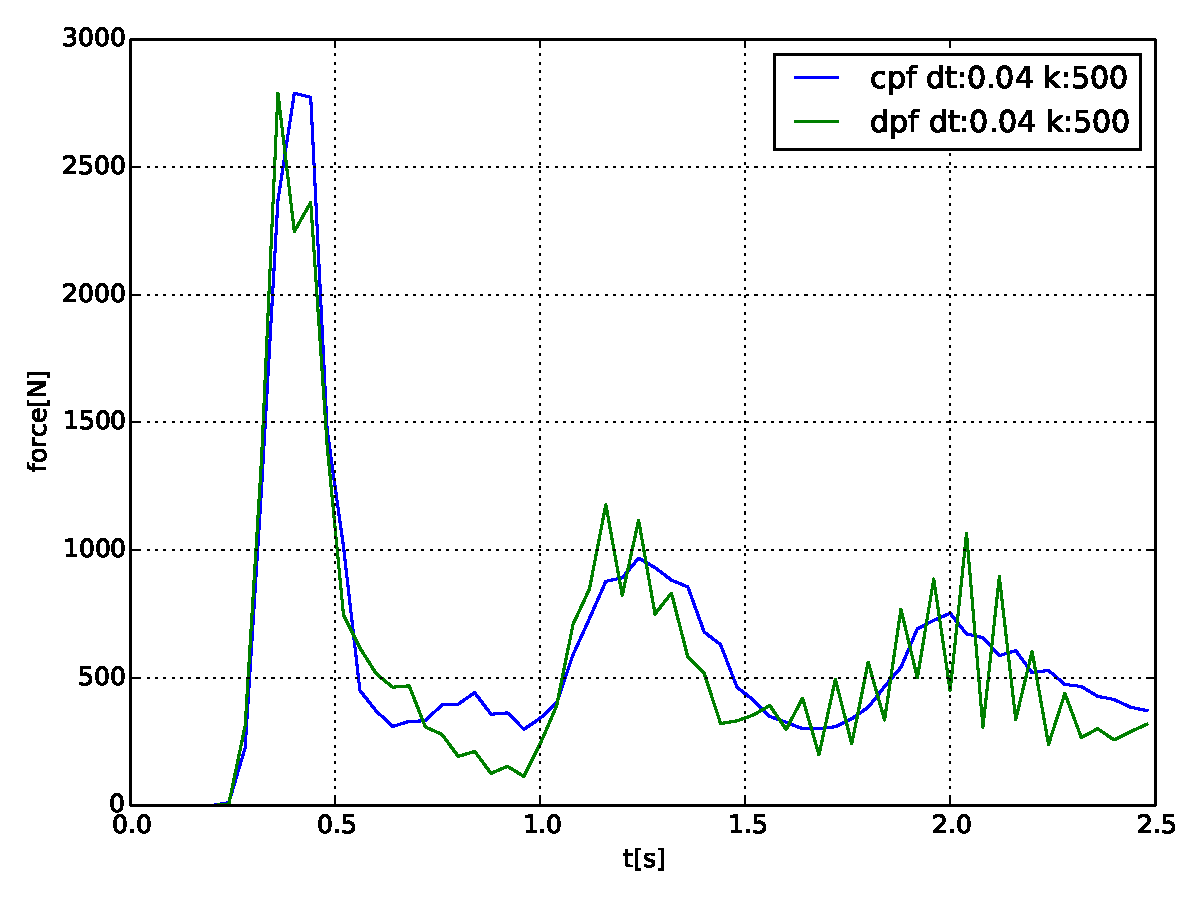
\includegraphics[width=1.0\textwidth]{pics/pdf/slidingVertexArtifactDiscretizationForcesRedefAlgo.pdf}
  \caption[2D-Illustration of the redefinition for a hooked collision.]{2D-Illustration of the redefinition for a hooked collision. 1) Neighboring triangles are candidates 2) Dismissal of the candidates with the vertex projection outside the triangle 3) Dismissal of the artifact candidates 4) Redefinition to the final candidate}
  \label{fig::slidingVertexArtifactDiscretizationForcesRedefAlgo}
\end{figure}
